\documentclass[11pt]{article}
\usepackage{v-test-paper}
\usepackage{mathtools}
%\usepackage{ifthen}
\title{Wave Mechanics}
\begin{document}
\maketitle

\begin{center}
    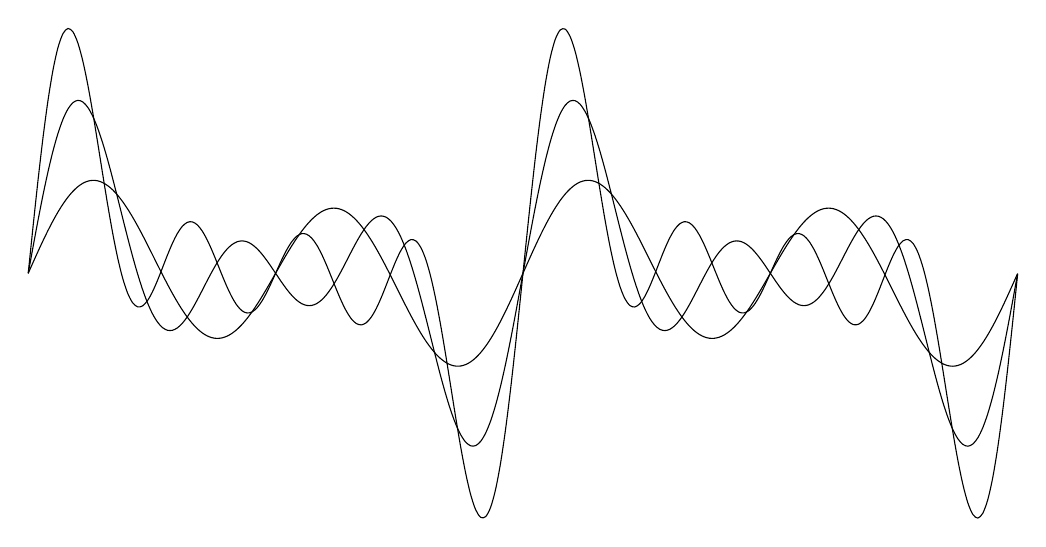
\begin{tikzpicture}
        % multiple sine cures with different frequencies and amplitudes between two points
            \draw[domain=0:4*pi, samples=200, smooth, variable=\x] plot ({\x}, {0.25*sin(deg(\x)) + sin(deg(2*\x))});
            \draw[domain=0:4*pi, samples=200, smooth, variable=\x] plot ({\x}, {0.5*sin(deg(\x)) + sin(deg(2*\x)) + sin(deg(3*\x))});
            \draw[domain=0:4*pi, samples=200, smooth, variable=\x] plot ({\x}, {0.75*sin(deg(\x)) + sin(deg(2*\x)) + sin(deg(3*\x)) + sin(deg(4*\x))});
            \tzcoor*(0, 0)(A)
            \tzcoor*(4*pi, 0)(B)
    \end{tikzpicture}
\end{center}


\begin{center}
    \begin{quote}
    \textit{A wave can be defined as a disturbance or variation that travels through a medium or space, transferring energy without permanently displacing the medium itself.}
    \end{quote}
\end{center}

\begin{itemize}
    \item \textbf{Partial derivatives}\\
    Let’s first talk about partial derivatives. Say you have a function of two parameters \( f(a, b) \). Now the parameters may be independent or dependent by a constraint equation. What a partial derivative means is that you differentiate the function \( f \) with respect to (one of) its variable keeping the other fixed.\\[2mm]So in the case of the wave function, taking a partial derivative with respect to time means you fix a position and look at how it varies in time. \\Similarly, a partial derivative with respect to space means you freeze an instant of time and look at the spatial variation of the function. Similarly, this can be extended for multiple partial derivatives. This can be seen as freezing time and following the dots over space.
    \begin{align*}
        \intertext{For simplicity in this article we used $\dfrac{\d{y}}{\d{x}}$ but it is actually $\dfrac{\partial{y}}{\partial{x}}$}
        \intertext{Similarly, $\dfrac{\d^2{y}}{\d{x^2}}$ is actually $\dfrac{\partial^2{y}}{\partial{x^2}}$}
    \end{align*}
    \begin{center}
        \begin{tikzpicture}
            \tzfn"curve"{sin(deg(\x))}[0:2*pi]
            \foreach \i in {0.1, 0.3,...,  2}{
                \tzvXpointat*{curve}{pi*\i}(A)
                \tzline+[->](A)(0, 0.5)
                \tzline+[->](A)(0, -0.5)
            }
            
        \end{tikzpicture}
    \end{center}

    \pagebreak
        \item \textbf{Wave Equation[1D]}
    \[ y = f\left(\textit{position of particle}, \textit{time}\right) \]
    \begin{center}
        \begin{tikzpicture}
            \def\dl{0.5}
            \def\X{2*pi}
            \def\LT{1}
            \def\F{sin(deg(\x))}
            \begin{scope}[xshift=1cm]
                \tzaxes(0, -1.5)(4.5*pi, 2)
                \tzfn\F[0:4*pi]
                \tzvXpointat{F}{\X}(A)
                \tzcircle(A)(15pt)
                \tzline+[->]($(A)+(0, -15pt)$)(0, -3)
            \end{scope}
            \begin{scope}[yshift=-8cm, scale=2, xshift=-2.5cm]
                \tzfn"arc"\F[\X-2*\LT:\X+2*\LT]
                \tzfn[line width=1mm]\F[\X - 0.5*\dl:\X + 0.5*\dl]
                \tzvXpointat{F}{\X}(A)
                %\tzcircle(A)(35pt) 
                \tzvXpointat*{F}{\X - 0.5*\dl}(START)
                \tzvXpointat*{F}{\X + 0.5*\dl}(END)
                \tztangent[->]"TL"{arc}(START)[\X-0.5*\dl:\X-\LT]{$T_1$}[b]
                \tztangent[->]"TR"{arc}(END)[\X+0.5*\dl:\X+\LT]{$T_2$}
                \tzline+[dashed](START)(-1, 0)
                \tzline+[dashed](START)(1, 0)
                \tzline+[dashed](END)(1, 0)
                \tzvXpointat{TR}{\X+1}(TRP)
                \tzanglemark($(START)+(1, 0)$)(START)(END){$\theta$}(8pt)
                \tzanglemark($(END)+(1, 0)$)(END)(TRP){$\theta + \d{\theta}$}[r](8pt)
                \tzline+[->](END)(1.5, 0){$T_2\cos(\theta+\d{\theta})$}[r]
                \tzline+[->](END)(0, 1.5){$T_2\sin(\theta+\d{\theta})$}[a]
                \tzline+[->](START)(0, -1.5){$T_1\sin(\theta)$}[b]
                \tzline+[->](START)(-1.5, 0){$T_1\cos(\theta)$}[l]
            \end{scope}
        \end{tikzpicture}
    \end{center}
    \begin{align*}
        \intertext{Above diagram shows a small segment of the string.}
        \intertext{Force along the horizontal direction will get balanced out, cause the string won't accelerate along horizontal.}
        T_2\cos(\theta+\d{\theta}) - T_1\cos(\theta) &= 0\\
        \Aboxed{T_1 &= T_2} \tag{1}\\
        \intertext{Force along the vertical direction won't be balanced out, cause the string will accelerate along vertical.}
        T_2\sin(\theta+\d{\theta}) - T_1\sin(\theta) &= m a_y\\
        \intertext{As string will perform small oscillations, $\theta$ will be small.}
        T_2\left(\theta + \d{\theta}\right) - T_1\theta &= m a_y\\
        \intertext{Also, the mass of this small segment will $\d{m}$,}
        T_2\left(\theta + \d{\theta}\right) - T_1\theta &= \d{m} a_y\\
        \intertext{Because of small oscillations length of this segment will be $\d{x}$ so, $\d{m} = \upmu \d{x}$, $T_1=T_2=T$}
        T_2\left(\theta + \d{\theta}\right) - T_1\theta &= \upmu \d{x} a_y\\
        T\d{\theta} &= \upmu \d{x} a_y\\
        \Aboxed{\dfrac{\d{\theta}}{\d{x}} &= \dfrac{\upmu}{T} a_y } \tag{2}\\
        \intertext{Also we have,}
        \dfrac{\d{y}}{\d{x}} &= \tan(\theta)\\
        \dfrac{\d^2{y}}{\d{x^2}} &= \sec^2\theta\dfrac{\d{\theta}}{\d{x}}\\
        \Aboxed{\dfrac{\d{\theta}}{\d{x}} &= \dfrac{\d^2{y}}{\d{x^2}}} \tag{3}\\
        \intertext{Combining both equations,}
        \dfrac{\d^2{y}}{\d{x^2}} &= \dfrac{\upmu}{T} a_y\\
        \intertext{As we know, $a_y = \dfrac{\partial^2{y}}{\partial{t^2}}$ and $\dfrac{\d^2{y}}{\d{x^2}}=\dfrac{\partial^2{y}}{\partial{x^2}}$}
        \Aboxed{\dfrac{\partial^2{y}}{\partial{x^2}} &= \dfrac{\upmu}{T} \dfrac{\partial^2{y}}{\partial{t^2}}} \tag{\textit{Wave Equation}}
    \end{align*}

    \item \textbf{Solution of above differential equation}
    \begin{align*}
        \intertext{Solving the above differential equation is beyond the scope of this article. But the solution is,}
        y(x, t) &= f\left(k x \pm \omega t\right)\\
        \intertext{Any function of the form $f\left(k x \pm \omega t\right)$ will satisfy the wave equation.}
        \intertext{Let's see what we get if we differentiate $y(x, t)$ with respect to $t$ and $x$.}
        \dfrac{\partial{y}}{\partial{t}} &= \pm \omega f'\left(k x \pm \omega t\right)\\
        \dfrac{\partial^2{y}}{\partial{t^2}} &= \omega^2 f''\left(k x \pm \omega t\right)\tag{1}\\
        \intertext{Similarly,}
        \dfrac{\partial{y}}{\partial{x}} &= k f'\left(k x \pm \omega t\right)\\
        \dfrac{\partial^2{y}}{\partial{x^2}} &= k^2 f''\left(k x \pm \omega t\right)\tag{2}\\
        \intertext{Substituting (1) and (2) in the wave equation,}
        k^2 f''\left(k x \pm \omega t\right) &= \dfrac{\upmu}{T} \omega^2 f''\left(k x \pm \omega t\right)\\
        \omega^2 &= \dfrac{\upmu}{T} k^2\\
        \Aboxed{\sqrt{\dfrac{T}{\upmu}} &= \dfrac{\omega}{k}} \\
    \end{align*}
    \pagebreak

    \item \textbf{Speed of wave}
    \begin{center}
        \begin{tikzpicture}
            \foreach \I [evaluate={\i=-\I*1.5}] in {0, 1,..., 5}{
                \tzcoor*(0, \i)(A)
                \tzcoor(10, \i)(B){$t=t_\I$}[r]
                \ifthenelse{\I=0}{\tzline+[<->]($(A)+(0, -0.5)$)(0, 1)}{}
                \tzline+(A)(-\i, 0)
                \tzfn<-\i, \i>{0.5*sin(deg(2*\x))}[0:0.5*pi]
                \tzline+(-\i + 0.5* pi, \i)(8+\i, 0)
                \tzline+[->]<0, 0.5>(-\i+0.25*pi, \i)(1, 0){$v$}[r]
            }
        \end{tikzpicture}
        \begin{tikzpicture}
            \def\dl{1}
            \def\X{0.5*pi}
            \def\LT{1.5}
            \def\F{sin(deg(\x))}
            \begin{scope}
                \tzfn"arc"\F[\X-2*\LT:\X+2*\LT]
                \tzfn[line width=1mm]\F[\X - 0.5*\dl:\X + 0.5*\dl]
                \tzvXpointat{F}{\X}(A)
                %\tzcircle(A)(35pt) 
                \tzvXpointat*{F}{\X - 0.5*\dl}(START)
                \tzvXpointat*{F}{\X + 0.5*\dl}(END)
                \tztangent[->]"TL"{arc}(START)[\X-0.5*\dl:\X-\LT]{$T_1$}[l]
                \tztangent[->]"TR"{arc}(END)[\X+0.5*\dl:\X+\LT]{$T_2$}[r]
                \tzvXpointat{TR}{\X+1}(TRP)
                \tzvXpointat{TL}{\X-1}(TLP)
                \tzanglemark($(START)+(-1, 0)$)(START)(TLP){$\theta$}(12pt)
                \tzanglemark'($(END)+(1, 0)$)(END)(TRP){$\theta$}[r](12pt)
                \tzline+[->](END)(1.5, 0){$T_2\cos(\theta)$}[r]
                %\tzline+[->](END)(0, -1.5){$T_2\sin(\theta+\d{\theta})$}[a]
                %\tzline+[->](START)(0, -1.5){$T_1\sin(\theta)$}[b]
                \tzline+[->](START)(-1.5, 0){$T_1\cos(\theta)$}[l]
                \tzline"RL"($(START)!0.01!(TLP)$)($(START)!1.2cm!90:($(START)!0.01!(TLP)$)$)
                \tzline"RR"($(END)!0.01!(TRP)$)($(END)!-1.2cm!90:($(END)!0.01!(TRP)$)$)
                \tzXpoint*{RL}{RR}(O)
                \tzanglemark(END)(O)(START){$2\theta$}(12pt)
            \end{scope}
            \begin{scope}[xshift=8cm]
                \tzfn"arc"\F[\X-2*\LT:\X+2*\LT]
                \tzfn[line width=1mm]\F[\X - 0.5*\dl:\X + 0.5*\dl]
                \tzvXpointat{F}{\X}(A)
                %\tzcircle(A)(35pt) 
                \tzvXpointat*{F}{\X - 0.5*\dl}(START)
                \tzvXpointat*{F}{\X + 0.5*\dl}(END)
                \tztangent[->]"TL"{arc}(START)[\X-0.5*\dl:\X-\LT]{$T_1$}[l]
                \tztangent[->]"TR"{arc}(END)[\X+0.5*\dl:\X+\LT]{$T_2$}[r]
                \tzline+[->](A)(1.5, 0){$v$}[r]
                \tzline+[->](A)(0, -1.5){$a_r$}[b]
            \end{scope}
        \end{tikzpicture}
    \end{center}
    \begin{align*}
        \intertext{As we can see in the above diagram, the wave is moving with a velocity $v$(actually the string is moving but in the case of mechanical wave it acts as a carrier of energy and momentum, hence we can assume speed of the wave will be same as the string) and the segment of string will have a radial acceleration($a_r$)}\\
        F_x &= 0\\
        F_y &= m a_r\\
        2T\sin\theta &= \dfrac{mv^2}{r}\\
        \intertext{As $\theta$ is small, $\sin\theta \approx \theta$}
        2T\theta &= \dfrac{\upmu \cdot r \cdot 2\theta v^2}{r}\\
        v^2 &= \dfrac{T}{\upmu}\\
        \Aboxed{v &= \sqrt{\dfrac{T}{\upmu}}}\tag{wave velocity}\\
        \intertext{Now, we can summarize the above discussion in a single equation,}
        \Aboxed{\dfrac{\partial^2{y}}{\partial{t^2}} = v^2\dfrac{\partial^2{y}}{\partial{x^2}}, \quad v = \sqrt{\dfrac{T}{\upmu}}, \quad v &=\dfrac{\omega}{k}=\dfrac{\textit{coefficient of time(t)}}{\textit{coefficient of space(x)}}}
    \end{align*}
    \pagebreak

    \item \textbf{Another look at wave velocity}
    \begin{center}
        \begin{tikzpicture}
            \tzaxes(0, -1)(4.5*pi, 2){$x$}{$y$}
            \tzfn"curve"{sin(deg(\x))}[0:4*pi]
            \foreach \x in {0.5*pi, 1.5*pi, 2.5*pi, 3.5*pi}{
                \tzvXpointat*{curve}{\x}(A)
                \tzline+[->](A)(1, 0){$v$}[r]
            }
            % \foreach \I [evaluate={\i=-\I*1.5}] in {0, 1, 2}{
            %     \tzcoor*(0, \i)(A)
            %     \tzcoor(10, \i)(B){$t=t_\I$}[r]
            %     \ifthenelse{\I=0}{\tzline+[<->]($(A)+(0, -0.5)$)(0, 1)}{}
            %     \tzline+(A)(-\i, 0)
            %     \tzfn<-\i, \i>{0.5*sin(deg(2*\x))}[0:0.5*pi]
            %     \tzline+(-\i + 0.5* pi, \i)(8+\i, 0)
            %     \tzline+[->]<0, 0.5>(-\i+0.25*pi, \i)(1, 0){$v$}[r]
            % }
        \end{tikzpicture}
    \end{center}
    \begin{align*}
        y(x, t) &= f\left(k x \pm \omega t + \phi\right)
        \intertext{For simplicity, let's assume a sine wave.}
        \intertext{Every peak is moving with a velocity $v$, this velocity is the velocity of the wave.}
        \intertext{This is the fun part, }
        \intertext{Rate at which peak is moving is $\dfrac{\d{x}}{\d{t}}$,}
        \intertext{To get peak, $kx \pm \omega t + \phi$ must be odd integral multiple of $\dfrac{\pi}{2}$,}
        kx \pm \omega t + \phi &= \left(2n+1\right)\dfrac{\pi}{2}
        \intertext{Differentiating both sides with respect to $t$,}
        k\dfrac{\d{x}}{\d{t}} \pm \omega &= 0\\
        \Aboxed{\dfrac{\d{x}}{\d{t}} &= \mp \dfrac{\omega}{k}}\\
        \intertext{This concludes an important result,}
    \end{align*}
    \vspace*{-60mm}
    \begin{center}
        \begin{tikzpicture}
            \tzaxes(0, -1)(4.5*pi, 1.5){$x$}{$y$}
            \tzfn"curve"{sin(deg(\x))}[0:4*pi]
            \foreach \x in {0.1, 0.2, ..., 4}{
                \tzvXpointat*{curve}{\x*pi}(A)
                \tzline+[->](A)(1, 0)
            }
        \end{tikzpicture}
    \end{center}
    \begin{align*}
        \intertext{Although we assumed only for peaks, but it is true for any point, because all the points are moving in the same fashion.}
        \intertext{For $y(x, t)=f(kx-\omega t + \phi)$, wave will move in the positive direction,}
        \Aboxed{v &= \dfrac{\omega}{k}}\\
        \intertext{For $y(x, t)=f(kx+\omega t + \phi)$, wave will move in the negative direction,}
        \Aboxed{v &= -\dfrac{\omega}{k}}
    \end{align*}

    \pagebreak

    \item \textbf{Longitudinal wave speed in different states of matter}
    \begin{center}
        \begin{quote}
        \textit{Longitudinal waves are waves in which the displacement of the medium is in the same direction as, or the opposite direction to, the direction of propagation of the wave. These displacements can be caused by variations in pressure, density, or state of the medium.}
        \end{quote}
    \end{center}

    \item \textbf{Relation between displacement wave and pressure wave}
    \begin{center}
        \begin{tikzpicture}
            \def\W{0.5}
            \begin{scope}
                \tzline(0, 0)(6, 0)
                \tzline(0, 2)(6, 2)
                \foreach \i in {1, 1.5, ..., 6}{
                    \tzrectangle+[pattern=north east lines](\i-\W, 0)(0.5*\W, 2)
                }
            \end{scope}
            \begin{scope}[xshift=8cm]
                \tzline(0, 0)(6, 0)
                \tzline(0, 2)(6, 2)
                \tzrectangle+[pattern=north east lines](2, 0)(\W, 2)
                \tznode(2+\W, 0){$x+\Delta x$}[br]
                \tznode(2, 0){$x$}[bl]
                \tzline+[|<->|]<0, 2.25>(2, 0)(\W, 0){$\Delta x$}[ma]
                \tzline+[dashed](2-\W, 0)(0, 2)
                \tzline+[->](2-2*\W, 1)(2*\W, 0){$p(x)$}[ma]
                \tzline+[->](2+5*\W, 1)(-4*\W, 0){$p(x+\Delta x)$}[ma]
                \tzline+[->](2-\W, -1)(3*\W, 0){$s(x, t)$}[mb]
                \tznode(6, 1){$A$}
            \end{scope}
        \end{tikzpicture}
    \end{center}
    Imagine sound wave moving across a pipe filled with air. Sound is a longitudinal wave, as the wave passes through the pipe, the air particles will move back and forth. \\[2mm]
    To visualize what's happening, imagine mentally dividing the air in the pipe, which is at rest if there is no sound, into a stack of thin slices. \\[2mm]
    Think about one of these slices. In equilibrium, it feels equal and opposite pressure from the gas on its two sides. As the sound wave goes through, the pressure wave generates slight differences in pressure on the two sides of our thin slice of air, and this imbalance of forces causes the slice to accelerate.\\
    
    In the above right diagram $s(x, t)$ is the displacement function across the pipe, $p(x)$ pressure at $x$ and $p(x+\Delta x)$ pressure at $x+\Delta x$ and $A$ is the cross-section area.\\
    
    Let's shortly discuss about the Bulk Modulus($B$),\\[2mm]
    The bulk modulus quantifies how resistant a substance is to changes in volume under the influence of an external pressure. Materials with high bulk modulus values are less compressible, meaning they experience smaller volume changes in response to applied pressure.
    \begin{center}
        \begin{tikzpicture}
            \tzrectangle+(0, 0)(3, 3)
            \tzrectangle+[dashed](0, 0)(3.5, 3)
            \tzline+[->](-1.5, 1.5)(1.5, 0){$p_L$}[ma]
            \tzline+[->](4.5, 1.5)(-1.5, 0){$p_R$}[ma]
        \end{tikzpicture}
    \end{center}
    \begin{align*}
        B &= -\dfrac{\Delta p}{\left(\dfrac{\Delta V}{V}\right)}\\
        \Delta p &= -B\dfrac{\Delta V}{V}
    \end{align*}
    Back to wave\_
    \pagebreak
    \begin{align*}
        \intertext{Now, we wanna inspect volume change across the segment of pipe,}
        \dfrac{\Delta V}{V} &= \dfrac{A\cdot s(x+\Delta x, t) - A\cdot s(x, t)}{A\cdot\Delta x}\\
             &= \dfrac{s(x+\Delta x, t) - s(x, t)}{\Delta x} \\
        \Aboxed{\dfrac{\Delta V}{V} &= \dfrac{\partial s(x, t)}{\partial x}}\\[2mm]
        \Aboxed{\Delta p &= -B\dfrac{\partial s(x, t)}{\partial x}}\\
        \intertext{This is the local pressure which is directly proportional to negative gradient of $s(x, t)$}
        \intertext{Now, we can apply Newton's second law for the segment of the pipe}
        F &= ma\\
        A\cdot \left( p(x, t) - p(x+\Delta x, t) \right) &= \left(A\cdot \Delta x \right)\cdot\uprho \dfrac{\partial^2s(x, t)}{\partial t^2}\\
        \intertext{put the expression for local pressure,}
        -B\dfrac{\partial s(x, t)}{\partial x} + B\dfrac{\partial s(x+\Delta x, t)}{\partial x} &= \left(\Delta x \right)\cdot\uprho \dfrac{\partial^2s(x, t)}{\partial t^2}\\[3mm]
        \dfrac{B\left(\dfrac{\partial s(x+\Delta x, t)}{\partial x}-\dfrac{\partial s(x, t)}{\partial x}\right)}{\Delta x} &= \uprho \dfrac{\partial^2s(x, t)}{\partial t^2}\\[3mm]
        \Aboxed{\dfrac{\partial^2s(x, t)}{\partial x^2} &=\dfrac{\uprho}{B} \dfrac{\partial^2s(x, t)}{\partial t^2}}\\  
        \intertext{Now, we can compare above equation with wave equation for string,}
        \dfrac{\partial^2y}{\partial x^2} &= \dfrac{1}{v^2} \dfrac{\partial^2y}{\partial t^2}\\[3mm]
        \Aboxed{v &= \sqrt{\dfrac{B}{\uprho}}}\\
        \intertext{This is the speed of longitudinal waves within a gas or a liquid.}\\[5mm]
        \intertext{Similarly, we can find out for solids,}
        \Aboxed{v &= \sqrt{\dfrac{Y}{\uprho}}}\\
        \intertext{$Y$ is Young's modulus of the solid and $\uprho$ is the density of the solid.}
    \end{align*}
    \pagebreak
    \item \textbf{Velocity of longitudinal wave in gases}

    \item \textbf{Energy and Power of a wave}
    \begin{center}
        \begin{tikzpicture}
            \tzfn"curve"{sin(deg(\x))}[0:pi]
            \tzfn[line width=0.5mm]{sin(deg(\x))}[0.2*pi:0.3*pi]
            \tzvXpointat*{curve}{pi*0.25}(A)
            \tzline+[->](A)(0, 0.5){$v_p$}[a]
            %\tzline+[->](A)(0, -0.5)
            \begin{scope}[xshift=6cm]
                \tzline+(0, 0)(2, 0){$\Delta x$}[mb]
                \tzline+(2, 0)(0, 0.5){$\Delta y$}[mr]
                \tzline(0, 0)(2, 0.5){$\Delta l$}[ma]
            \end{scope}
        \end{tikzpicture}
    \end{center}
    \begin{center}
        \begin{quote}
            \textit{In the context of a string wave, consider the movement of a segment of the string. As this segment oscillates, it possesses kinetic energy, quantifiable by the formula $\dfrac{1}{2}mv^2$. However, there is an additional phenomenon at play: the string segment also undergoes slight elongation, resulting in potential energy. Each element behaves as a temporary spring, and the potential energy can be calculated using $\int\vec{F}\cdot\d{\vec{s}}$. The total energy of the segment is the sum of the kinetic and potential energies.}
        \end{quote}
        \[ y(x, t) = A\sin\left(kx-\omega t\right) \]
    \end{center}
    \begin{align*}
        \intertext{Kinetic energy of the segment,}
        K.E. &= \dfrac{1}{2}m v_p^2 \\
            &= \int \dfrac{1}{2}\d{m}\left(\dfrac{\partial y}{\partial t}\right)^2\\
            &= \dfrac{1}{2}\left(\upmu\d{x} \right)\left(\dfrac{\partial y}{\partial t}\right)^2\\
            &= \int \dfrac{1}{2} \upmu A^2\omega^2 \cos^2\left(kx-\omega t\right) \d{x}\\
        \intertext{We can calculate average kinetic energy over one complete oscillation,}
        <K.E.> &= \dfrac{1}{2} \upmu A^2\omega^2\int_0^\lambda \cos^2\left(kx-\omega t\right) \d{x}\\ 
                &=\dfrac{1}{2} \upmu A^2\omega^2\int_0^\lambda \dfrac{\left(1 + \cos\left(2\left(kx-\omega t\right)\right)\right)}{2} \d{x}\\  
                &= \dfrac{1}{4} \upmu A^2\omega^2 \left[x + \dfrac{\sin\left(2kx-2\omega t\right)}{2k}\right]_0^\lambda\\
                &= \dfrac{1}{4} \upmu A^2\omega^2 \left[\lambda + \dfrac{\sin\left(2k\lambda-2\omega t\right)-\sin\left(-2\omega t\right)}{2k}\right]\\
                &= \dfrac{1}{4} \upmu A^2\omega^2 \left[\lambda + \dfrac{\sin\left(4\pi-2\omega t\right)+\sin\left(2\omega t\right)}{2k}\right]\\  
                &= \dfrac{1}{4} \upmu A^2\omega^2 \left[\lambda + \dfrac{2*\sin\left(2\pi\right)*\cos\left(4\pi-4\omega t\right)}{2k}\right]\\ 
                &= \dfrac{1}{4} \upmu A^2\omega^2 \lambda
    \end{align*}
    \pagebreak
    \begin{align*}
        \intertext{Potential energy of the segment,}\\
        \intertext{Firstly, we have to calculate the elongation in the segment using above right diagram}
        \Delta l &= \sqrt{\Delta x^2 + \Delta y^2} - \Delta x\\
            &= \Delta x\sqrt{1 + \left(\dfrac{\Delta y}{\Delta x}\right)^2} - \Delta x
            \intertext{As string will perform small oscillations $\dfrac{\Delta y}{\Delta x}$ will be small}
            &= \Delta x \left(1+\dfrac{1}{2} \left(\dfrac{\Delta y}{\Delta x}\right)^2\right) - \Delta x\\
        \Delta l &\approx \dfrac{1}{2}\left(\dfrac{\Delta y}{\Delta x}\right)^2 \Delta x
    \end{align*}
    \begin{align*}
        \intertext{As $\dfrac{\Delta y}{\Delta x}$ is slope hence, $\dfrac{\partial y}{\partial x}$,}
        U &= \int T \cdot \dfrac{1}{2} \left(\dfrac{\partial y}{\partial x}\right)^2 \d{x}\\
        &= \int \dfrac{1}{2} T A^2k^2 \cos^2\left(kx-\omega t\right) \d{x}\\
        \intertext{Again, we can calculate average potential energy over one complete oscillation,}
        <U> &= \dfrac{1}{2}TA^2k^2\int_0^\lambda  \cos^2\left(kx-\omega t\right) \d{x}
        \intertext{From above integration we got $\lambda/2$ and $\omega = \sqrt{\dfrac{T}{\upmu}}k$}
        <U> &= \dfrac{1}{4}\upmu A^2\omega^2\lambda
        \intertext{So, total energy in one complete oscillation will be,}
        \textit{Total Energy} &= K.E. + U\\
        \Aboxed{E &= \dfrac{1}{2}\upmu A^2\omega^2 \lambda}
        \intertext{Total energy per unit length will be like,}
        \dfrac{E}{\lambda} &= \dfrac{1}{2}\upmu A^2\omega^2\\
        \Aboxed{u &= \dfrac{1}{2}\upmu A^2\omega^2}
    \end{align*}

    
    \pagebreak
\end{itemize}
\pagebreak
\begin{center}
    \textbf{Superposition of waves}
    \begin{quote}
        \textit{When two or more waves travel in the same medium, they are bound to interact with each other. They retain their wave nature after combining with each other, but usually, the resultant wave is different from both of the individual waves. The superposition principle helps us describe the resulting wave or motion that is produced when two or more waves combine with each other. }
    \end{quote}
\end{center}
\begin{itemize}
    \item Two sin waves with different frequencies but same amplitudes\\
    \begin{tikzpicture}
        \begin{scope}
            \tzaxes(0, -1)(2.25*pi, 1.5){$x$}{$y_2$}
            \tzfn{sin(deg(2*\x))}[0:2*pi]
        \end{scope}
        \begin{scope}[yshift=4cm]
            \tzaxes(0, -1)(2.25*pi, 1.5){$x$}{$y_1$}
            \tzfn{sin(deg(\x))}[0:2*pi]
        \end{scope}
        \tznode(2.5*pi, 2){$\Rightarrow$}
        \begin{scope}[xshift=9cm, yshift=2cm]
            \tzaxes(0, -1)(2.25*pi, 2){$x$}{$y_1+y_2$}
            \tzfn{sin(deg(\x)) + sin(deg(2*\x))}[0:2*pi]
        \end{scope}
    \end{tikzpicture}
    
    \item Two sin waves with same frequencies but different amplitudes\\
    \begin{tikzpicture}
        \begin{scope}
            \tzaxes(0, -1)(2.25*pi, 1.5){$x$}{$y_2$}
            \tzfn{0.5*sin(deg(2*\x))}[0:2*pi]
        \end{scope}
        \begin{scope}[yshift=4cm]
            \tzaxes(0, -1)(2.25*pi, 1.5){$x$}{$y_1$}
            \tzfn{sin(deg(2*\x))}[0:2*pi]
        \end{scope}
        \tznode(2.5*pi, 2){$\Rightarrow$}
        \begin{scope}[xshift=9cm, yshift=2cm]
            \tzaxes(0, -1)(2.25*pi, 2){$x$}{$y_1+y_2$}
            \tzfn{sin(deg(2*\x)) + 0.5*sin(deg(2*\x))}[0:2*pi]
        \end{scope} 
    \end{tikzpicture}

    \item Two sin waves with different frequencies and amplitudes\\
    \begin{tikzpicture}
        \begin{scope}
            \tzaxes(0, -1)(2.25*pi, 1.5){$x$}{$y_2$}
            \tzfn{0.5*sin(deg(2*\x))}[0:2*pi]
        \end{scope}
        \begin{scope}[yshift=4cm]
            \tzaxes(0, -1)(2.25*pi, 1.5){$x$}{$y_1$}
            \tzfn{sin(deg(3*\x))}[0:2*pi]
        \end{scope}
        \tznode(2.5*pi, 2){$\Rightarrow$}
        \begin{scope}[xshift=9cm, yshift=2cm]
            \tzaxes(0, -1)(2.25*pi, 2){$x$}{$y_1+y_2$}
            \tzfn{sin(deg(3*\x)) + 0.5*sin(deg(2*\x))}[0:2*pi]
        \end{scope} 
    \end{tikzpicture}

    \begin{center}
        \begin{quote}
            \textit{In reality, waves are not limited to simple sinusoidal waves. They can be any shape, and the superposition principle applies to all of them.\\[2mm]
            Almost all waves(continuous and differentiable) can be described as a superposition of simpler waves, means that the wave can be broken down into a sum of sinusoidal waves.}
        \end{quote}
        \begin{tikzpicture}
            \begin{scope}
                \tzaxes(0, -1)(2.25*pi, 1.25){$x$}{$y_3$}
                \tzfn{sin(deg(8*\x))}[0:2*pi]
            \end{scope}
            \begin{scope}[yshift=3cm]
                \tzaxes(0, -1)(2.25*pi, 1.25){$x$}{$y_2$}
                \tzfn{sin(deg(4*\x))}[0:2*pi]
            \end{scope}
            \begin{scope}[yshift=6cm]
                \tzaxes(0, -1)(2.25*pi, 1.25){$x$}{$y_1$}
                \tzfn{sin(deg(2*\x))}[0:2*pi]
            \end{scope}
            \tznode(2.5*pi, 3){$\Rightarrow$}
            \begin{scope}[xshift=9cm, yshift=3cm]
                \tzaxes(0, -2)(2.25*pi, 3){$x$}{$y_1+y_2+y_3$}
                \tzfn{sin(deg(2*\x)) + sin(deg(4*\x)) + sin(deg(8*\x))}[0:2*pi]
            \end{scope} 
        \end{tikzpicture}
    \end{center}

    \item \textbf{Resultant Amplitude and Intensity due to two coherent waves}\\
    \textbf{Coherent Waves }: \textit{Two waves are said to be coherent if their frequencies are same. But actually we define coherence of wave according to phase difference, means there should be a constant phase difference for the waves to be coherent.}

    \begin{itemize}
        \item \textbf{resultant amplitude}
        \begin{align*}
            y_1 &= A_1 \sin(kx-\omega t + \phi_1)\\
            y_2 &= A_2 \sin(kx-\omega t + \phi_2)\\
            y &= y_1 + y_2\\
            y &= A_1 \sin(kx-\omega t + \phi_1) + A_2 \sin(kx-\omega t + \phi_2)\\
                &= A_1 \sin(kx-\omega t) \cos(\phi_1) + A_1 \cos(kx-\omega t) \sin(\phi_1) + \\ &\quad A_2 \sin(kx-\omega t) \cos(\phi_2) + A_2 \cos(kx-\omega t) \sin(\phi_2)\\
                &= \sin(kx-\omega t) \underbrace{(A_1 \cos(\phi_1) + A_2 \cos(\phi_2))}_{A\cos(\phi)} + \cos(kx-\omega t) \underbrace{(A_1 \sin(\phi_1) + A_2 \sin(\phi_2))}_{A\sin(\phi)}\\
              \Aboxed{y  &= A \sin(kx-\omega t + \phi)}\\
        \end{align*}
        \begin{align*}
            A\cos(\phi) &= A_1 \cos(\phi_1) + A_2 \cos(\phi_2)\\
            A\sin(\phi) &= A_1 \sin(\phi_1) + A_2 \sin(\phi_2)\\
            \intertext{Squaring and adding both the equations,}
            A^2\cos^2(\phi) + A^2\sin^2(\phi) &= (A_1 \cos(\phi_1) + A_2 \cos(\phi_2))^2 + (A_1 \sin(\phi_1) + A_2 \sin(\phi_2))^2\\
            A^2 &= A_1^2 + A_2^2 + 2A_1A_2(\cos(\phi_1)\cos(\phi_2) + \sin(\phi_1)\sin(\phi_2))\\
            A^2 &= A_1^2 + A_2^2 + 2A_1A_2\cos(\phi_1 - \phi_2)\\
            \Aboxed{A &= \sqrt{A_1^2 + A_2^2 + 2A_1A_2\cos(\phi_1 - \phi_2)}}\\
            \intertext{Also, one more relation we can derive from the above equations,}
            \tan(\phi) &= \frac{A_1 \sin(\phi_1) + A_2 \sin(\phi_2)}{A_1 \cos(\phi_1) + A_2 \cos(\phi_2)}\\
            \Aboxed{\phi &= \tan^{-1}\left(\frac{A_1 \sin(\phi_1) + A_2 \sin(\phi_2)}{A_1 \cos(\phi_1) + A_2 \cos(\phi_2)}\right)}\\
        \end{align*}
        \begin{center}
            \begin{tikzpicture}
                \tzline[->](0, 0)(4, 0){$\vec{A_1}$}[r]
                \tzline[->](0, 0)(2, 3){$\vec{A_2}$}[a]
                \tzline[->](0, 0)(5, 3){$\vec{A}$}[a]
                \tzanglemark(2, 0)(0, 0)(5, 3){$\phi$}(35pt)
                \tzanglemark(4, 0)(0, 0)(2, 3){$\Delta \phi$}(15pt)
                \tznode(2.5, -1){\textit{also we can analyze the resultant amplitude using vector method}}
            \end{tikzpicture}
        \end{center}
        \item \textbf{resultant intensity}
        \begin{align*}
            \intertext{from the equation for intensity,}
            I &= \frac{1}{2} \rho \omega^2 A^2 v\\
            I &\propto A^2\\
            A^2 &= A_1^2 + A_2^2 + 2A_1A_2\cos(\phi_1 - \phi_2)\\
            \Aboxed{I &= I_1 + I_2 + 2\sqrt{I_1I_2}\cos(\phi_1 - \phi_2)}\\
            \intertext{Special case, when $A_1=A_2=A_0$}
            A^2 &= A_0^2 + A_0^2 + 2A_0^2\cos(\phi_1 - \phi_2)\\
            A^2 &= 2A_0^2 + 2A_0^2\cos(\phi_1 - \phi_2)\\
            A^2 &= 2A_0^2(1 + \cos(\phi_1 - \phi_2))\\
            \Aboxed{A &= 2A_0\cos\left(\frac{\Delta \phi}{2}\right)}\\[2mm]
            \Aboxed{A_{\textit{max}} &= 2A_0}\\
            \intertext{If $A_1=A_2=A_0 \rightarrow I_1=I_2=I_0$ }
            I &= 2I_0 + 2I_0\cos(\phi_1 - \phi_2)\\
            I &= 2I_0(1 + \cos(\phi_1 - \phi_2))\\
            \Aboxed{I &= 4I_0\cos^2\left(\frac{\Delta \phi}{2}\right)}\\[2mm]
            \Aboxed{I_{\textit{max}} &= 4I_0}\\
        \end{align*}
        \pagebreak
        \item \textbf{maximization and minimization of intensity}
        \begin{align*}
            I &= I_1 + I_2 + 2\sqrt{I_1I_2}\cos(\Delta \phi)\\
            \intertext{For maximum intensity, $\cos(\Delta \phi) = 1$, for minimum intensity, $\cos(\Delta \phi) = -1$}
            I_{\textit{max}} &= I_1 + I_2 + 2\sqrt{I_1I_2}\\
                            &= \left(\sqrt{I_1} + \sqrt{I_2}\right)^2\\[5mm]
            I_{\textit{min}} &= I_1 + I_2 - 2\sqrt{I_1I_2}\\
                            &= \left(\sqrt{I_1} - \sqrt{I_2}\right)^2\\
        \end{align*}
    \end{itemize}

\end{itemize}






\end{document}